\documentclass[tikz,border=8pt]{standalone}

\usepackage[T1]{fontenc}
\usepackage[utf8]{inputenc}
\usepackage{lmodern}
\usepackage{amssymb}
\usepackage{tikz}
\usetikzlibrary{arrows.meta,positioning,fit,calc,backgrounds}

\begin{document}
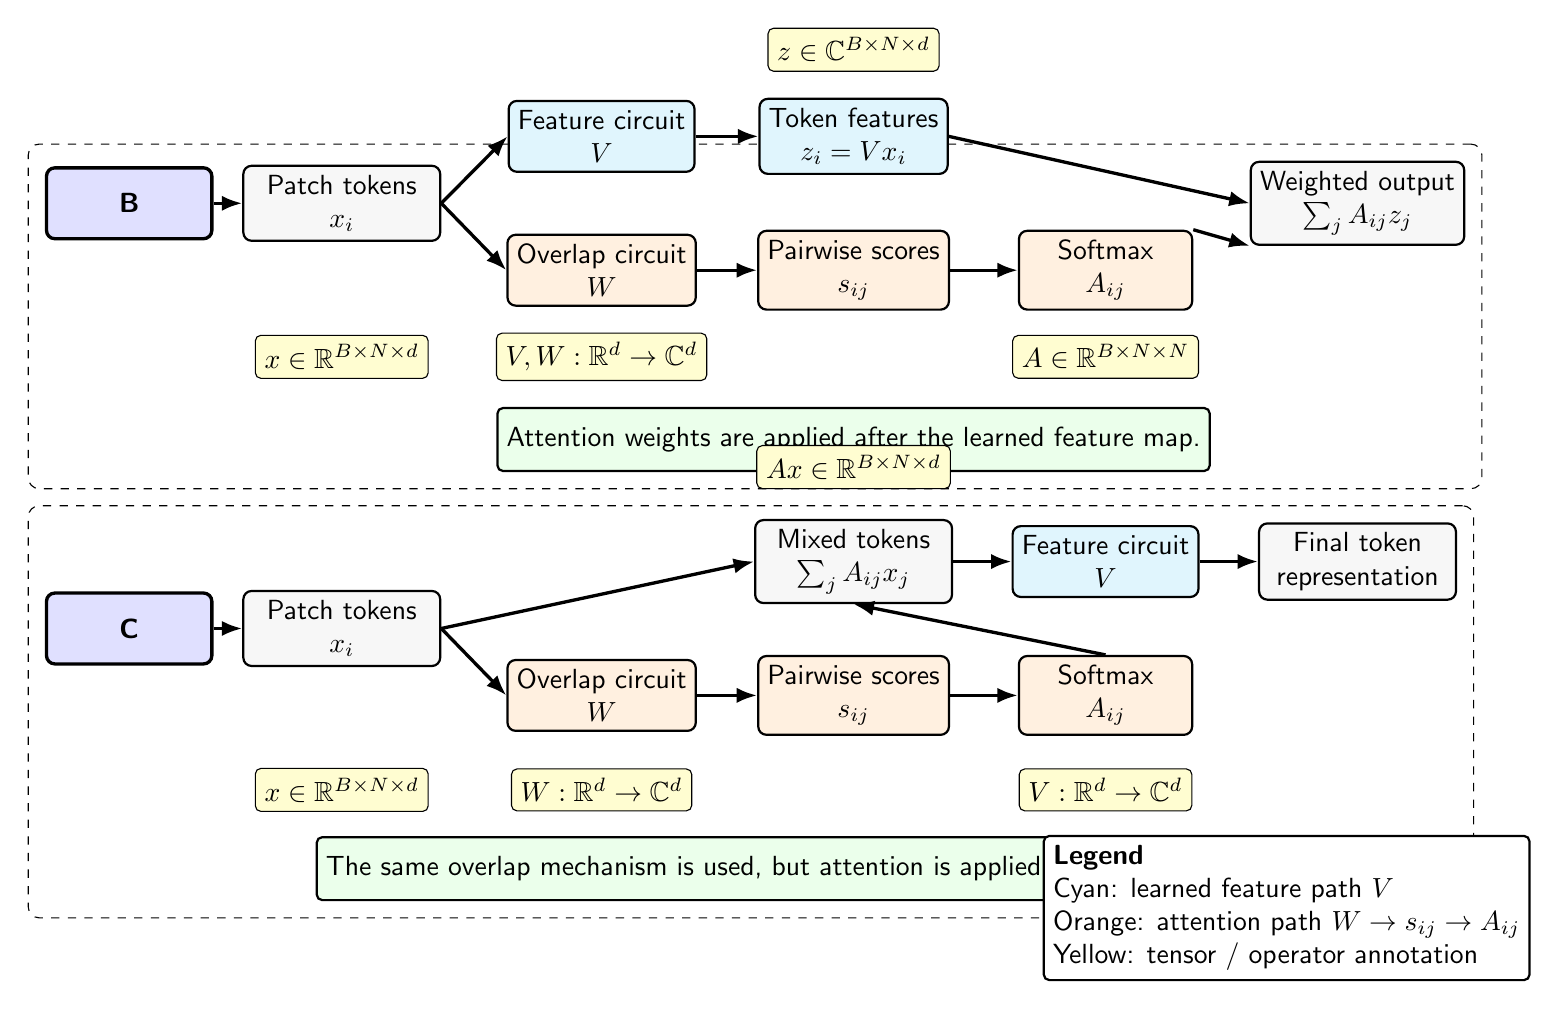
\begin{tikzpicture}[
  font=\sffamily,
  x=1cm, y=1cm,
  title/.style={draw, rounded corners=3pt, minimum width=2.1cm, minimum height=0.9cm, align=center, fill=blue!12, very thick},
  block/.style={draw, rounded corners=3pt, minimum width=2.5cm, minimum height=0.95cm, align=center, fill=gray!6, thick},
  feat/.style={draw, rounded corners=3pt, minimum width=2.2cm, minimum height=0.85cm, align=center, fill=cyan!12, thick},
  attn/.style={draw, rounded corners=3pt, minimum width=2.2cm, minimum height=0.85cm, align=center, fill=orange!12, thick},
  ann/.style={draw, rounded corners=2pt, minimum width=2.1cm, minimum height=0.5cm, align=center, fill=yellow!18, thin},
  note/.style={draw, rounded corners=2pt, minimum width=4.4cm, minimum height=0.8cm, align=center, fill=green!8, thick},
  legend/.style={draw, rounded corners=2pt, minimum width=5.0cm, minimum height=0.8cm, align=left, fill=white, thick},
  arrow/.style={-{Latex[length=2.6mm]}, very thick},
  dashedbox/.style={draw, dashed, rounded corners=4pt, inner sep=6pt}
]

\node[title] (btitle) at (1.3, 0) {\textbf{B}};
\node[block] (bx) at (4.0, 0) {Patch tokens\\$x_i$};
\node[feat]  (bv) at (7.3, 0.85) {Feature circuit\\$V$};
\node[attn]  (bw) at (7.3, -0.85) {Overlap circuit\\$W$};
\node[feat]  (bz) at (10.5, 0.85) {Token features\\$z_i = Vx_i$};
\node[attn]  (bs) at (10.5, -0.85) {Pairwise scores\\$s_{ij}$};
\node[attn]  (ba) at (13.7, -0.85) {Softmax\\$A_{ij}$};
\node[block] (bout) at (16.9, 0) {Weighted output\\$\sum_j A_{ij} z_j$};
\node[ann] (bsh1) at (4.0, -1.95) {$x \in \mathbb{R}^{B\times N\times d}$};
\node[ann] (bsh2) at (7.3, -1.95) {$V,W:\mathbb{R}^{d}\rightarrow\mathbb{C}^{d}$};
\node[ann] (bsh3) at (10.5, 1.95) {$z \in \mathbb{C}^{B\times N\times d}$};
\node[ann] (bsh4) at (13.7, -1.95) {$A \in \mathbb{R}^{B\times N\times N}$};
\node[note]  (bnote) at (10.5, -3.0) {Attention weights are applied after the learned feature map.};

\node[title] (ctitle) at (1.3, -5.4) {\textbf{C}};
\node[block] (cx) at (4.0, -5.4) {Patch tokens\\$x_i$};
\node[attn]  (cw) at (7.3, -6.25) {Overlap circuit\\$W$};
\node[attn]  (cs) at (10.5, -6.25) {Pairwise scores\\$s_{ij}$};
\node[attn]  (ca) at (13.7, -6.25) {Softmax\\$A_{ij}$};
\node[block] (cmix) at (10.5, -4.55) {Mixed tokens\\$\sum_j A_{ij} x_j$};
\node[feat]  (cv) at (13.7, -4.55) {Feature circuit\\$V$};
\node[block] (cout) at (16.9, -4.55) {Final token\\representation};
\node[ann] (csh1) at (4.0, -7.45) {$x \in \mathbb{R}^{B\times N\times d}$};
\node[ann] (csh2) at (7.3, -7.45) {$W:\mathbb{R}^{d}\rightarrow\mathbb{C}^{d}$};
\node[ann] (csh3) at (10.5, -3.35) {$A x \in \mathbb{R}^{B\times N\times d}$};
\node[ann] (csh4) at (13.7, -7.45) {$V:\mathbb{R}^{d}\rightarrow\mathbb{C}^{d}$};
\node[note]  (cnote) at (10.5, -8.45) {The same overlap mechanism is used, but attention is applied before the final feature map.};

\node[legend] (leg) at (16.0, -8.95) {\textbf{Legend}\\Cyan: learned feature path $V$\\Orange: attention path $W \rightarrow s_{ij} \rightarrow A_{ij}$\\Yellow: tensor / operator annotation};

\draw[arrow] (btitle.east) -- (bx.west);
\draw[arrow] (bx.east) -- (bv.west);
\draw[arrow] (bx.east) -- (bw.west);
\draw[arrow] (bv.east) -- (bz.west);
\draw[arrow] (bw.east) -- (bs.west);
\draw[arrow] (bs.east) -- (ba.west);
\draw[arrow] (bz.east) -- (bout.west);
\draw[arrow] (ba.north east) -- (bout.south west);

\draw[arrow] (ctitle.east) -- (cx.west);
\draw[arrow] (cx.east) -- (cw.west);
\draw[arrow] (cw.east) -- (cs.west);
\draw[arrow] (cs.east) -- (ca.west);
\draw[arrow] (cx.east) -- (cmix.west);
\draw[arrow] (ca.north) -- (cmix.south);
\draw[arrow] (cmix.east) -- (cv.west);
\draw[arrow] (cv.east) -- (cout.west);

\begin{scope}[on background layer]
  \node[dashedbox, fit=(btitle) (bout) (bnote)] {};
  \node[dashedbox, fit=(ctitle) (cout) (cnote)] {};
\end{scope}
\end{tikzpicture}
\end{document}
